\section{Planning}
\label{Planning}

We begonnen het project met het maken van een planning voor de komende tien
weken zodat er voor zowel de opdrachtegever als onszelf duidelijk was wanneer
er wat gedaan zou worden. In verband met de Agile methoden zijn de eerste paar
weken in meer detail gepland dan de latere weken met de bedoeling om de
planning steeds bij te werken voor de komende (paar) weken. Deze voorgenomen
planning wordt besproken in paragraaf \ref{voorgenomen_planning}. Voor een
uitgebreidere beschrijving van de diverse fasen kan het Plan van Aanpak uit de
bijlage worden bekeken. Zoals verwacht is deze ruwe planning aangepast in de
weken daarna, deze realisatie wordt besproken in \ref{werkelijke_planning}.

\subsection{Voorgenomen planning}
\label{voorgenomen_planning}

Doordat we in het begin slechts een grove planning hebben gemaakt waren vooral
de eerste paar weken in detail uitgewerkt. Er moesten twee documenten af zijn
voordat er met de implementatie van het product kon worden begonnen, dit zijn
het plan van aanpak (PvA) en het requirement analysis document (RAD). Tevens
hebben we ons direct voorgenomen een demo in de eerste weken van het project te
maken zodat de opdrachtgever snel feedback kon geven op de richting waar het
project in gaat.
Aangezien de tentamens op 16/06 beginnen is afgesproken
voor deze datum het project af te ronden. In de onderstaande Ganntchart wordt
de planning zichtbaar gemaakt zoals wij het aan het begin van het project
voorstelden.

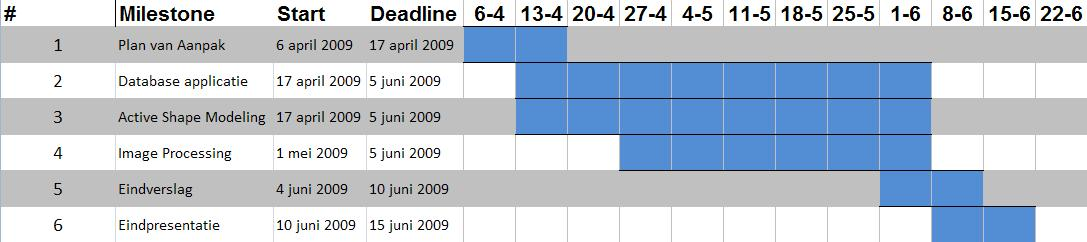
\includegraphics[width=0.8\textwidth]{ganntbefore}

\subsubsection{Plan van Aanpak}

Tijdens ons eerste gezamelijk overleg is het volgende schema voor het PvA
afgesproken, waarbij de deadlines zijn gemaakt met de gelegenheid om
verbeteringen door te voeren in het achterhoofd.

09/04: Concept PvA mailen
14/04: Verwerken feedback PvA
15/04: Meeting in erasmus
17/04: PvA af

\subsubsection{Requirement Analysis Document}

Tevens is voor het RAD een (minder granulaire) planning gemaakt, deze overlapt
met de planning voor het PvA gezien het schrijven van het tweede document en
het verwerken van verbeteringen aan een ander document tegelijk kunnen worden
uitgevoerd.

Nadat de tweede ronde van feedback op het PvA was verwerkt werd begonnen met
het RAD, zodat deze zo snel mogelijk afgerond kon worden en aan de
implementatie kon worden begonnen. Eventuele feedback op het PvA hierna werdt
eerst verwerkt.

27/04: RAD af

\subsubsection{Database Applicatie}

Om een demo te kunnen geven waarin zo veel mogelijk ge\"{e}valueerd kan worden
over de gewenste functionaliteiten was besloten om de twee weken na het
inleveren van het RAD te besteden aan het maken van spike solutions en deze te
integreren in een simpele applicatie die de basisfunctionaliteiten aan de
opdrachtgever presenteert.

08/05: Database Applicatie af

\subsubsection{Active Shape Modelling}

Een belangrijk deel van de applicatie is het weergeven van de hoofdmodi van
variatie per landmark type en het weergeven van de gemiddelde landmarks.

25/05: Active Shape Modelling af

\subsubsection{Image Processing}

Aanvankelijk zagen we deze fase als het projecteren van resultaten op
bijvoorbeeld r\"{o}ntgenfoto's. In de loop van het project hebben we de
betekenis van deze fase echter verandert in het tekenen van gebieden en
morphen van deze gebieden naar een gemiddeld been. Dit is een cruciale fase
voor de aangeboden oplossing.

11/06: Image Processing af

\subsubsection{Eindverslag}

Het schrijven van het eindverslag moet ruim voor de eindpresentatie afgerond
zijn zodat het verslag goedgekeurd kan worden voor aanvang van de eindpresentatie.

12/06 Eindverslag af

\subsubsection{Eindpresentatie}

De eindpresentatie is de uiteindelijke afronding van het project.

19/06: Eindpresentatie gegeven

\subsection{Werkelijke planning}
\label{werkelijke_planning}

In deze sectie geven wij aan hoe de opgestelde planning aansluit op de
uiteindelijke realisatie.

Zowel het PvA als het RAD zijn op tijd af gekomen, de andere milestones zijn
wat gewijzigd. Aangezien verschillende leden van de projectgroep tentamens
hebben in de weken vanaf 15 juni is besloten om het project rond deze datum af
te ronden. Hierdoor schoven de deadlines voor het schrijven van het eindverslag
en het geven van de eindpresentatie op naar voren.

In de originele planning is hierdoor naar 10 juni verschoven en de
eindpresentatie zal op 15 juni plaatsvinden.  Door een goede scheiding van de
verschillende functionaliteiten bleek het goed mogelijk om een werkverdeling te
maken waar iedereen zijn of haar expertisegebieden in kwijt kon. Hierdoor
liepen de Database Applicatie, Active Shape Model en Image Processing fasen
parallel aan elkaar en werden de laatste werkzaamheden tegelijk afgerond.

In de latere weken van het project bleek ook nog enige tijd nodig om de code te
refactoren, bugs te verwijderen en functionaliteiten verder te verbeteren. Dit
zorgde ervoor dat de eerdergenoemde drie parallel-lopende fasen wat uitliepen.

In de originele planning was geen rekening gehouden met de tijd die nodig is om
de applicatie ook te laten draaien op een server in het Erasmus MC. Hierdoor
moet dit tegelijk plaatsvinden met het schrijven van het verslag.

In de onderstaande Ganntchart is te zien hoe de werkelijke planning verliep:

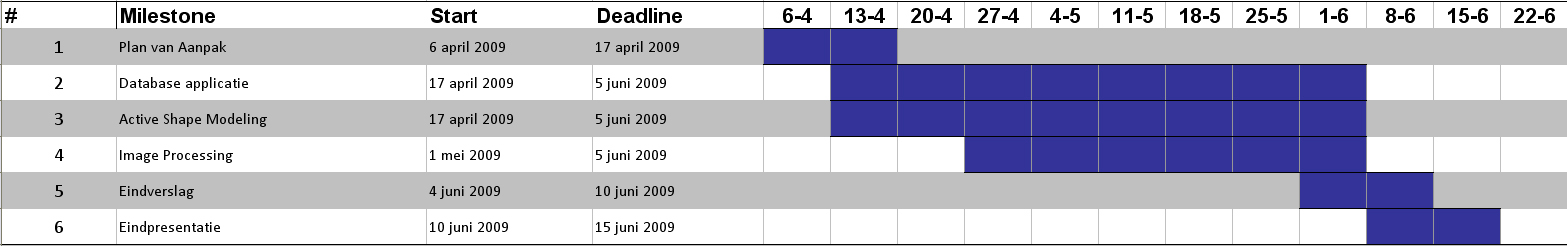
\includegraphics[width=0.8\textwidth]{ganntafter}
